\documentclass[10pt,conference]{IEEEtran}
\IEEEoverridecommandlockouts
% The preceding line is only needed to identify funding in the first footnote. If that is unneeded, please comment it out.
\usepackage{cite}
\usepackage{amsmath,amssymb,amsfonts}
\usepackage{algorithmic}
\usepackage{graphicx}
\usepackage{textcomp}
\usepackage{xcolor}

\usepackage{array}
\usepackage{float}
\usepackage{hyperref}
\usepackage{makecell}
\usepackage{changepage}
\usepackage{fontawesome}
\usepackage{subcaption}
\usepackage{booktabs}
\usepackage{rotating}
\usepackage{xspace}
\usepackage{xcolor}
\usepackage{microtype}
\usepackage{multirow}
\usepackage{comment}
\usepackage[normalem]{ulem}
\usepackage[inkscapelatex=false]{svg}
\usepackage{tabularx}
\usepackage{siunitx}
\usepackage[inline]{enumitem}
\usepackage{tcolorbox}
\usepackage{listings}

\def\BibTeX{{\rm B\kern-.05em{\sc i\kern-.025em b}\kern-.08em
    T\kern-.1667em\lower.7ex\hbox{E}\kern-.125emX}}
\begin{document}

\title{
GreenMeasurer: a Non-Intrusive Framework to Measure the Energy Consumption of Software Systems
}


\author{\IEEEauthorblockN{Simão Cunha}
\IEEEauthorblockA{\textit{INESC TEC \& University of Minho} \\
Braga, Portugal \\
simao.s.cunha@inesctec.pt}
\and
\IEEEauthorblockN{João Saraiva}
\IEEEauthorblockA{\textit{INESC TEC \& University of Minho} \\
Braga, Portugal \\
saraiva@di.uminho.pt}
}

\maketitle

\begin{abstract}
This tool paper presents GreenMeasurer, a practical and extensible open-source framework for non-intrusively measuring the energy consumption of software systems on Linux and macOS. GreenMeasurer captures energy metrics for CPU and GPU hardware domains without requiring source code modifications. Hardware support is implemented as plugins behind a common CPU/GPU interface: the CPU and GPU backends are selected independently at run time, and a metric whose backend is missing or unsupported is reported explicitly as unavailable instead of aborting the run. The tool integrates configurable temperature calibration, system condition management and, on Intel CPUs, optional power capping into an automated pipeline with a standard (per-run) and an over-time (time series) mode. Adding support for a new CPU or GPU only requires a new backend directory, with no change to the core.
\end{abstract}

\begin{IEEEkeywords}
Energy Measurement, Green Computing, Linux, macOS, Intel RAPL, NVIDIA NVML, Power capping
\end{IEEEkeywords}


\section{Introduction}

\textcolor{red}{ATUALIZAR ESTE PAPER DE ACORDO COM O NOVO README DE 5 DE FEVEREIRO DE 2026}
The energy consumption of software systems has become a central concern in modern computing, driven by the growing deployment of applications across energy-constrained environments such as mobile devices, embedded systems and large-scale cloud infrastructures. Software is now recognized as a major contributor to the overall energy footprint of computing systems, influencing not only performance and operating costs but also environmental sustainability \cite{10.1007/s10664-013-9276-6, 10.1145/3154384}. Accurate measurement of software energy consumption is therefore essential for understanding how design decisions, programming languages and runtime behaviors affect energy efficiency \cite{10.1145/2168836.2168841, 10.1145/2568225.2568297}. 

To address these challenges, the GreenMeasurer framework provides a practical and extensible environment for non-intrusively measuring the energy consumption and execution time of software programs in two ways: \begin{enumerate*}[label=(\arabic*), itemjoin={{; }}, itemjoin*={{; and }}]
    \item measuring both metrics immediately before and after program execution
    \item continuously measuring both metrics throughout the program's runtime
\end{enumerate*}.


GreenMeasurer reads the energy counters exposed by the hardware through \emph{backends}. The current backends use Intel's \textit{Running Average Power Limit} (RAPL) \cite{intel-rapl-reporting, 10.1145/3177754} interface through Model-Specific Registers (MSRs) for Intel CPUs and integrated GPUs, NVIDIA's NVML for NVIDIA GPUs and, on macOS, \texttt{powermetrics} for Apple Silicon. CPU and GPU backends are chosen independently at run time, so a machine with an unsupported CPU and a supported GPU (or the opposite) still yields the metrics that can be measured, and the others are reported as unsupported. Measurements are hardware-domain measurements, not per-process attributions.

GreenMeasurer contributes the following main features:
\begin{itemize}
    \item Hardware-level energy monitoring: Measures energy consumption of the CPU (e.g., Package, Core, DRAM) and the GPU, according to the backends available on the machine;
    \item Easy to use and easy to extend: the user supplies a command and a few parameters, and support for a new CPU or GPU is added as a self-contained backend directory, with no change to the core (Section~\ref{sec:adding_backend});
    \item Graceful degradation: a missing or unsupported backend never aborts a run; its metrics are written as \texttt{NOT\_SUPPORTED};
    \item Language-agnostic operation: Supports any executable program - binary, bytecode or source code - without requiring instrumentation or modifications to the source code;
    \item Measurement modes: Offers three complementary modes: 
    \begin{itemize}
        \item Standard - measures overall energy and execution time per run;
        \item Perf - collects detailed CPU performance counters;
        \item Over-time - continuously records energy consumption and CPU temperature during execution.
    \end{itemize}
    \item Automated calibration and validation: Includes CPU temperature calibration to ensure consistent thermal conditions and allows configurable variance thresholds to improve measurement reliability;
    \item Power capping support: Available only on Intel CPUs, where it integrates with the Linux Powercap library \cite{powercap2025} to impose predefined power limits. The tool validates this at run time and refuses a capped run when the selected CPU backend does not support it.
\end{itemize}

Originally developed and validated in previous research works \cite{10.1145/3136014.3136031, PEREIRA2021102609,10.1145/3687997.3695638}, this repository has been recently updated to include full parameterization of all execution arguments, a plugin-based backend architecture, support for NVIDIA GPUs and macOS, and a module for system power capping \cite{powercap2025} on Intel CPUs.

To address the challenges of accurately quantifying software energy consumption, we developed GreenMeasurer, a lightweight and extensible framework designed to provide repeatable energy measurements on Linux and macOS machines. GreenMeasurer measures hardware energy consumption of the CPU and GPU components through the backends available on the machine. It supports any type of program - whether distributed as binaries, bytecode or source code - without requiring modifications to the application's implementation. To enhance measurement reliability, the framework automatically controls system conditions, such as disabling Wi-Fi, to minimize external interference and measurement noise. Each experiment includes CPU temperature calibration and validation phases to ensure consistent thermal conditions across runs. Additionally, GreenMeasurer offers optional system power capping to facilitate energy-performance trade-off analysis and produces detailed measurement logs in CSV format for subsequent statistical processing. Finally, it includes a runtime monitoring feature that continuously records the energy consumption of the \textit{Package}, \textit{Core}, \textit{DRAM} and \textit{GPU}, along with CPU temperature, enabling time-based analysis of these metrics and generating an additional CSV file with the over-time measurements. Currently, it supports three complementary measurement modes that address different analysis needs: \textit{standard} measurements capture overall energy consumption and execution time per run; \textit{perf} measurements collect detailed CPU performance counters; and \textit{over-time} measurements record energy and temperature evolution during execution. Together, these modes provide both aggregate and fine-grained perspectives on software energy behavior.

GreenMeasurer has certain limitations. CPU energy is currently measured on Intel processors (RAPL through MSRs \cite{msr4}) and on Apple Silicon (\texttt{powermetrics}); support for AMD processors is left as future work. The macOS backends are implemented but have not yet been validated on hardware. Power capping \cite{powercap2025} is available only on Linux with Intel CPUs. The tool is not intended for containerized or virtualized environments, and network and I/O energy consumption cannot be measured separately from total system consumption.

To ensure measurement reliability, the framework includes internal validation mechanisms. Users can calibrate a baseline CPU temperature, after which executions are allowed only if the current temperature remains at or below the baseline plus a configurable variance threshold. For over-time measurements, the CPU temperature must consistently stay at or below the value recorded during the calibration process. Programs can also be re-executed multiple times to mitigate the effects of outliers \cite{castor2024estimatingenergyfootprintsoftware} and a configurable timeout prevents excessively long runs.

To demonstrate GreenMeasurer's capabilities, this paper presents example results obtained through its execution. We utilized GreenMeasurer to analyze the C implementation of the recursive Fibonacci algorithm in C. This analysis aims to illustrate GreenMeasurer's effectiveness in tasks such as measuring the energy consumption and execution time of multiple hardware components (\textit{Package}, \textit{Core}, \textit{DRAM} and \textit{GPU}) of any software without modifying its source code, continuously monitoring energy consumption and execution time throughout the program's runtime, and evaluating the impact of power capping on software energy consumption and runtime in Linux systems with Intel CPUs. The paper also describes how a new backend is added (Section~\ref{sec:adding_backend}) and plans a comparison with CodeCarbon and EnergiBridge (Section~\ref{sec:eval_plan}).

The following sections describe related work (Section \ref{rw_section}), the design of GreenMeasurer (Section \ref{sec:greenmeasurer}), demonstrate its usage through practical experiments (Section \ref{demo_section}) and discuss conclusions and future directions (Section \ref{conc_section}).

\begin{tcolorbox}[colback=gray!10!white, colframe=black!60, arc=4pt, boxrule=0.5pt]
\centering
\faGithub\ \textbf{All collected data and source code are available at:}\\[3pt]
\href{https://github.com/simaocunha71/GreenMeasurer}{\texttt{https://github.com/simaocunha71/GreenMeasurer}}
\end{tcolorbox}

\section{Related Work}
\label{rw_section}

Accurately measuring software energy consumption has been a longstanding research challenge, leading to the development of various tools that differ in methodology, level of abstraction and target environments.

Several approaches provide language-specific libraries for energy measurement. For instance, pyRAPL \cite{pyrapl} exposes Intel's RAPL counters through a simple Python interface, while jRAPL \cite{jRAPL} enables energy profiling for Java programs. These tools allow fine-grained energy monitoring directly within the program but require source code modifications and are limited to their respective programming ecosystems. In contrast, GreenMeasurer is language-agnostic and operates externally to the target program, avoiding the need for instrumentation.

Other tools aim for higher-level abstractions, often estimating the environmental impact of software execution. CodeCarbon \cite{benoit_courty_2024_11171501}, for example, estimates $CO_{2}$ emissions and energy consumption across hardware components such as CPU, RAM and GPU. While useful for assessing carbon footprints, such estimation-based tools rely on model approximations when low-level measurement interfaces are unavailable, which can compromise precision.

Recent tools such as Scaphandre \cite{Scaphandre} and Kepler \cite{10254956} address software energy monitoring in modern and containerized environments. Scaphandre collects energy data from Intel RAPL interfaces and exports metrics through Prometheus, enabling system-wide energy monitoring with minimal configuration. Kepler integrates with Kubernetes to estimate pod-level energy consumption based on performance counters and hardware telemetry, providing visibility into energy usage across containers and workloads.

GreenMeasurer, on the other hand, focuses on repeatable measurements of a command, without instrumentation, on bare-metal machines. It reads hardware counters directly and automates temperature calibration, repeated executions and (on Intel CPUs) power capping, which has been used in prior studies. Although it does not support containerized or virtualized systems, this design enables simpler setup, making it particularly suitable for experimental and comparative studies of software energy consumption.

We compare GreenMeasurer with two tools: CodeCarbon \cite{benoit_courty_2024_11171501}, a Python library that is integrated into the program under test, and EnergiBridge, a cross-platform command-line tool that measures the energy of a command from hardware counters. \textbf{[TODO: confirm the description, supported platforms and add the reference of EnergiBridge.]} GreenMeasurer's positioning rests on the following properties, each with its justification:

\begin{itemize}
    \item \textbf{Ease of use.} A command and a few parameters are enough; no code change is needed and the same workflow applies to any language.
    \item \textbf{Ease of extension.} A new CPU or GPU is supported by adding one backend directory (Section~\ref{sec:adding_backend}); the core, the build and the CSV schema adapt automatically.
    \item \textbf{Graceful degradation.} CPU and GPU backends are selected independently; an unsupported one yields \texttt{NOT\_SUPPORTED} instead of an abort or a silent estimate.
    \item \textbf{Testable hardware support.} The backend interface allows fake backends, so the selection and fallback logic is verified by an automated test suite without needing every hardware combination (these tests check orchestration, not counter accuracy).
    \item \textbf{Self-describing output.} Each backend declares its metrics (name, unit, kind, scope) and the CSV header is generated from them, so the output cannot drift from what the hardware provides. A missing value is never written as zero.
    \item \textbf{Controlled conditions.} Temperature calibration and the disabling of Wi-Fi during runs address known sources of variation in energy measurements. Whether they reduce variance is to be shown experimentally (Section~\ref{sec:eval_plan}).
    \item \textbf{Small dependency footprint.} The core is plain C with \texttt{dlopen}; optional libraries only affect the backend that needs them.
\end{itemize}

All measurements are hardware-domain measurements (package, core, DRAM, GPU) and not per-process attributions, so they include activity outside the target command.

\section{The GreenMeasurer Framework}
\label{sec:greenmeasurer}

GreenMeasurer is a framework developed to support the measurement of software energy consumption using the hardware energy counters exposed by CPUs and GPUs. It automates the configuration, execution and collection of energy metrics, aiming to make energy profiling practical and reproducible for software developers and researchers. It runs on Linux (Intel CPUs and integrated GPUs, NVIDIA GPUs) and macOS (Apple Silicon).

\subsection{Overview}

The framework combines a set of Bash scripts, C utilities and Makefiles to form a reproducible measurement pipeline that requires minimal user intervention; it does not require modifying source code to measure the energy consumption of a program.

The general architecture is shown in Figure~\ref{architecture_diagram}, which illustrates the workflow of the framework. First, the framework is executed with the appropriate arguments configured for the experiment. The next step is \textit{CPU temperature calibration}: the system is left idle for a specified number of seconds (it is executed a \textit{sleep} command), during which the average temperature of all CPU cores is recorded using the \textit{lm-sensors} library \cite{lm-sensors} and stored in a text file. Optionally, a \textit{power cap calibration} can be performed. In this step, a custom program (for example, the provided Python implementation of the Fibonacci algorithm) is executed across a range of power caps. A Python script then analyzes the resulting CSV file to identify the optimal power cap, defined here as the value that minimizes \textit{Package} energy consumption. After calibration, the framework can perform either over-time measurements or standard repeated executions. In the over-time mode, the target program is executed while continuously logging, at a user-defined interval, the energy metrics of the selected backends along with CPU temperature. In the standard mode, the framework first performs a series of idle runs for a specified number of seconds (executes a \textit{sleep} command), repeated \textit{n\_times} times, to establish the baseline energy consumption of the system under minimal load. Only after completing these idle measurements is the target program executed, with all results appended to the CSV file \texttt{measurements.csv}. The purpose of the idle runs is to isolate the program's energy consumption from the system's baseline energy usage. Each entry in this CSV file starts with the fields below, followed by one column per metric declared by the selected backends (named \texttt{<category>.<name>\_<unit>}, Table~\ref{table:metrics}):

\begin{itemize}
    \item \textbf{Language} - Programming language label (text).
    \item \textbf{Program} - Program name label (text).
    \item \textbf{Powercap} - Power cap value applied (W), or $-1$ if none.
    \item \textbf{Time\_ms} - Execution time (ms).
    \item \textbf{CPU\_Memory\_KB} - Peak resident memory of the command (KiB), measured in a separate run.
\end{itemize}

An unavailable value is written as \texttt{NOT\_SUPPORTED}, never as zero.

\begin{figure*}[!ht]
    \centering
    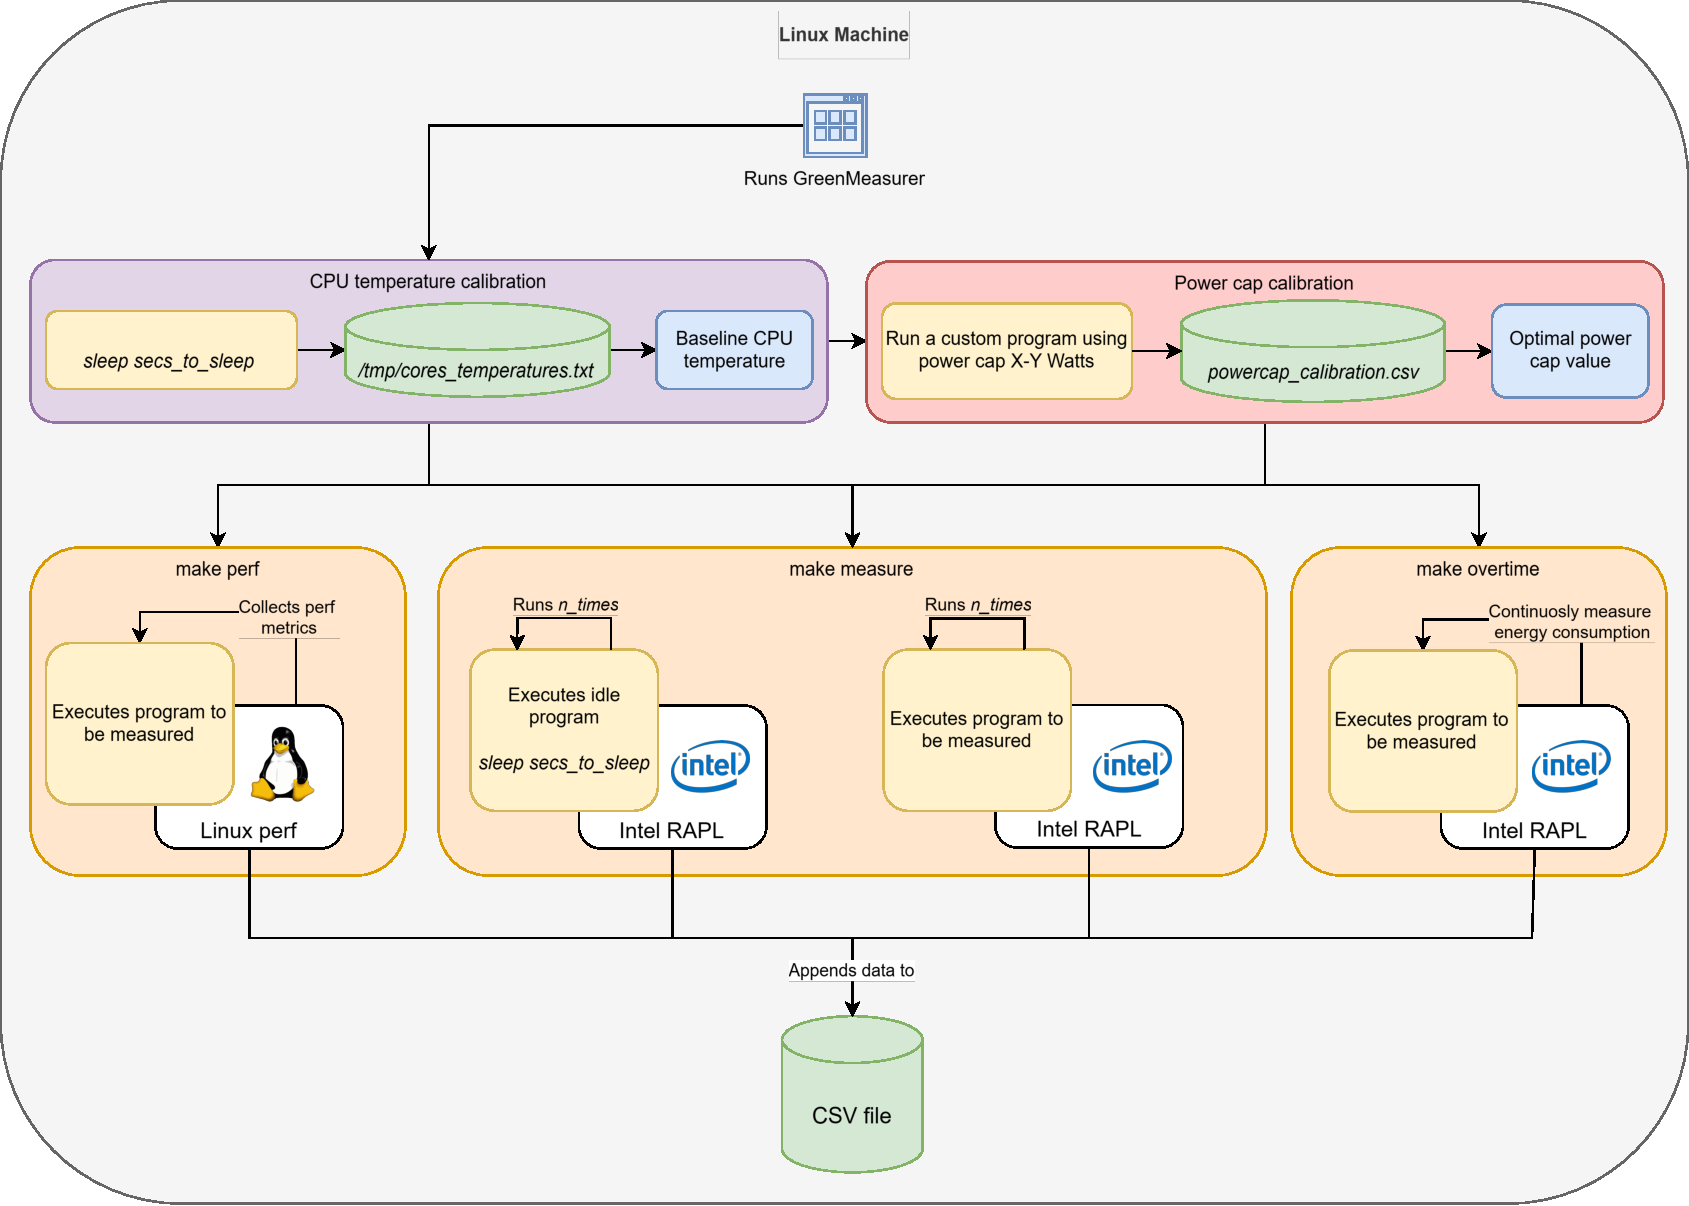
\includegraphics[width=\linewidth]{images/architecture.pdf}
    \caption{GreenMeasurer Architecture}
    \label{architecture_diagram}
\end{figure*}

In Table \ref{table:arguments}, we present the parameters of \textit{GreenMeasurer}, many of which are shared by the \textit{standard} mode, \textit{over-time} measurements (Section~\ref{overtime_section}) and the two calibration modes (Section~\ref{calibration_modes_section}).

\begin{table*}[t]
    \centering
    \caption{Command-line options of GreenMeasurer. All modes accept \texttt{-command} (the command to run through \texttt{/bin/sh -c}).}
    \label{table:arguments}
    \small
    \begin{tabularx}{\textwidth}{@{}l l l X@{}}
        \toprule
        \textbf{Option} & \textbf{Unit/type} & \textbf{Modes} & \textbf{Meaning} \\
        \midrule
        \texttt{-language} & text & all & Label written to the \texttt{Language} column; it does not change how the command runs. \\
        \texttt{-program} & text & all & Label written to the \texttt{Program} column. \\
        \texttt{-n\_times} & count & std.\ (1), cal.\ (3) & Number of measured runs (per power limit in calibration). \\
        \texttt{-variance} & \si{\celsius} & all & Maximum temperature above the calibrated baseline at which a run may start; otherwise the tool waits, checking every second (defaults: 0 standard, 5 over-time and calibration). Skipped if no CPU temperature is available. \\
        \texttt{-time\_out\_limit} & hours & std., cal. & Time limit of the initial check run; on expiry a \texttt{TimeOut} row is recorded (default 1). \\
        \texttt{-interval} & ms & over-time & Time between samples (default 100). \\
        \texttt{-powercap} & W, or $-1$ & std., over-time & Package power limit (Intel only); $-1$ means no cap (default); otherwise at least 1. \\
        \texttt{-sleep\_time}, \texttt{-sleep-secs} & s & all & Idle time used to settle the machine when a temperature baseline has to be created (default 5; 10 as \texttt{-secs\_to\_sleep} in calibration). \\
        \texttt{-calib-file} & path & all & Baseline-temperature file (default \texttt{/tmp/cores\_temperatures.txt}). \\
        \texttt{-output} & path & all & Output CSV (defaults \texttt{measurements.csv}, \texttt{measurements\_ot.csv}, \texttt{powercap\_calibration.csv}). \\
        \texttt{-range} & \texttt{min-max}, W & cal. & Range of power limits to test; the minimum is 1 W. \\
        \texttt{-compile\_cmd} & text & cal. & Optional command run once before the sweep. \\
        \bottomrule
    \end{tabularx}
\end{table*}

\begin{table*}[t]
    \centering
    \caption{Output metrics. A \emph{window} metric is the difference of a counter between the start and the end of the run (cumulative since the start in over-time mode); a \emph{gauge} is a single reading; a \emph{peak} is the highest reading seen while the command ran.}
    \label{table:metrics}
    \small
    \begin{tabularx}{\textwidth}{@{}l l l l X@{}}
        \toprule
        \textbf{Column} & \textbf{Unit} & \textbf{Kind} & \textbf{Backend} & \textbf{Meaning} \\
        \midrule
        \texttt{Time\_ms} & ms & core & all & Duration of the run (\texttt{Timestamp\_ms}: time since start, in over-time mode). \\
        \texttt{CPU\_Memory\_KB} & KiB & core & all & Peak resident memory of the command (separate run). \\
        \texttt{cpu.Package\_J} & J & window & Intel & Energy of the CPU package. \\
        \texttt{cpu.Core\_J} & J & window & Intel & Energy of the cores (part of the package). \\
        \texttt{cpu.DRAM\_J} & J & window & Intel & Energy of the memory. \\
        \texttt{cpu.Temperature\_C} & \si{\celsius} & gauge & Intel & Average core temperature. \\
        \texttt{cpu.CPU\_J}, \texttt{cpu.ANE\_J} & J & window & Apple & CPU and Neural Engine energy from \texttt{powermetrics}. \\
        \texttt{gpu.GPU\_J} & J & window & NVIDIA, Intel, Apple & GPU energy. \\
        \texttt{gpu.Power\_W} & W & gauge & NVIDIA & Instantaneous GPU power. \\
        \texttt{gpu.Temperature\_C} & \si{\celsius} & gauge & NVIDIA, Intel & GPU temperature. \\
        \texttt{gpu.Utilization\_\%} & \% & gauge & NVIDIA & GPU utilization. \\
        \texttt{gpu.VRAM\_MiB} & MiB & peak & NVIDIA & GPU memory used by the process. \\
        \bottomrule
    \end{tabularx}
\end{table*}

\subsection{Backends}
\label{sec:backends}

The core (\texttt{main.c}) handles the command line, orchestration, sampling, calibration and CSV output, and contains no hardware-specific code. Hardware support lives in \emph{backends}: shared objects (\texttt{backend.so}) placed under \texttt{platform/<os>/cpu/<name>} or \texttt{platform/<os>/gpu/<name>}. At startup the core loads each \texttt{backend.so}, validates its exported descriptor, calls its \texttt{detect()} function, and selects the detected backend with the highest priority in each category. One CPU backend and one GPU backend are chosen independently. If a category has no usable backend, its metrics are written as \texttt{NOT\_SUPPORTED} and the run continues; only when neither category is usable does the tool exit with an error. The backend directory can be overridden with \texttt{GREENMEASURER\_BACKEND\_DIR}, and \texttt{GREENMEASURER\_VERBOSE\_BACKENDS=1} lists the state of every backend (\texttt{selected}, \texttt{available}, \texttt{not detected}, \texttt{not built}, \texttt{load failed}, \texttt{invalid}). Table~\ref{table:backends} lists the existing backends.

\begin{table}[t]
    \centering
    \caption{Backends in the repository.}
    \label{table:backends}
    \small
    \begin{tabularx}{\columnwidth}{@{}l l X@{}}
        \toprule
        \textbf{Type} & \textbf{Backend} & \textbf{Source / status} \\
        \midrule
        CPU & Intel & RAPL MSRs; temperature; power capping \\
        CPU & AMD Zen & MSRs; not validated, future work \\
        CPU & Apple Silicon & \texttt{powermetrics}; not yet validated \\
        GPU & Intel integrated & RAPL PP1 MSR \\
        GPU & NVIDIA & NVML total-energy counter \\
        GPU & Apple Silicon & \texttt{powermetrics}; not yet validated \\
        \bottomrule
    \end{tabularx}
\end{table}

\subsection{Adding a Backend}
\label{sec:adding_backend}

A backend implements the interface in \texttt{energy-backend.h}: a \texttt{detect} function, \texttt{init}/\texttt{cleanup}, \texttt{sample\_start}/\texttt{sample\_stop} (the measurement window), a table of metric descriptors (name, unit, kind and scope) and a \texttt{get\_metric} function, plus an exported \texttt{energy\_backend\_descriptor} with its category and priority. Power capping is optional for CPU backends. The repository includes two complete, working examples, TOY\_CPU and TOY\_GPU (in \texttt{examples/toy\_backends}), whose energy values are fake by design. TOY\_CPU declares \texttt{cpu.Energy\_J} (window) and \texttt{cpu.LoadAvg\_1m} (gauge); TOY\_GPU declares \texttt{gpu.Energy\_J}, \texttt{gpu.Power\_W} and \texttt{gpu.Memory\_MiB}. Each is a single C file of about one hundred lines, built with \texttt{make -C examples/toy\_backends} and loaded without touching the core by setting \texttt{GREENMEASURER\_BACKEND\_DIR}. Moving the directory into \texttt{src/platform/} makes the standard build pick it up. The CSV columns of the new metrics appear automatically.

\subsection{System Requirements}

GreenMeasurer runs on Linux and on macOS (Apple Silicon). The \texttt{src/Makefile} selects \texttt{platform/linux} or \texttt{platform/macos} according to the operating system. Reading the energy counters requires root privileges. On Linux the Intel backends use RAPL through the \texttt{msr} kernel module; CPU temperature is read with \textit{lm-sensors} \cite{lm-sensors}; the Intel power-capping support uses \textit{powercap} \cite{powercap2025} and \textit{raplcap} \cite{raplcap}; the NVIDIA backend needs the NVML header and library at build time. A missing optional dependency only skips the backend that needs it. On macOS there are no RAPL or MSR counters, so the Apple backends run \texttt{powermetrics} in the background and integrate the average power it reports in each sampling interval (100 ms by default) into energy; the energy is thus known only to within one sampling interval. There is no power capping and no CPU temperature on macOS. The helper scripts that disable Wi-Fi are Linux-only. On Linux, a dedicated setup script installs the dependencies (\textit{i.e.} \textit{raplLibrariesSetup.sh}).

\subsection{Makefile Integration}

To evaluate a software system, a dedicated \textit{Makefile} must exist that defines a common set of targets for compilation, execution and measurement. This structure provides a uniform interface across heterogeneous environments and simplifies experiment automation.

The standard targets are:
\begin{itemize}
    \item \texttt{compile} - builds the program using the corresponding compiler or interpreter;
    \item \texttt{run} - executes the compiled or interpreted program with a parametrized input;
    \item \texttt{standard} - runs the program and collects energy and runtime data with the selected backends;
    \item \texttt{overtime} - runs the program and collects energy data with the selected backends during the program's execution time (see Section \ref{overtime_section});
    \item \texttt{clean} - removes all generated binaries and temporary files.
\end{itemize}

This Makefile-based design ensures consistent measurement behavior across all programs, allowing researchers to reproduce experiments by invoking the same target. 

\subsection{Calibration Modes}
\label{calibration_modes_section}

To improve the reliability of the collected data, GreenMeasurer supports two calibration modes.

The \textit{temperature calibration} mode measures the average temperature of CPU cores by executing a \textit{sleep} command for a specified number of seconds (\textit{secs\_to\_sleep} argument from Table \ref{table:arguments}). It then records the average temperature of all cores using the \textit{lm-sensors} library. Whenever a program is about to run, the CPU temperature must be below or equal to the baseline temperature plus a user-defined temperature variance (\textit{variance} from Table \ref{table:arguments}), otherwise a \textit{sleep} command of one second is executing until the condition is met. This mode can be executed as follows:

\begin{verbatim}
sudo ./main --temperature-calibration -sleep-secs 20
\end{verbatim}

The \textit{power cap calibration} mode iteratively tests different power cap values to determine the most energy-efficient setting (least \textit{Package} energy consumption) for a given workload. Power capping is available only on Intel CPUs, and the tool validates this at run time: if the selected CPU backend has no power-capping support (e.g., no Intel CPU), calibration and capped runs abort with an error instead of silently running uncapped. Power capping has been used in previous studies \textbf{[cite]}. Users provide a custom program for testing - for example, the GreenMeasurer repository includes a recursive Fibonacci algorithm in Python located in the \texttt{Utils/} folder. This mode can be executed as follows (where \textit{min} and \textit{max} define the range of power cap values, \textit{compile\_cmd} is the compilation command for the custom program - omit if using an interpreted language - and \textit{run\_cmd} is the execution command):

Both calibration modes are designed to make energy measurements more reproducible. The temperature calibration ensures similar CPU conditions across runs, while power cap calibration automatically finds the most efficient power limit for a certain system. This combination helps minimize measurement noise and allows consistent comparisons across experiments.

\begin{verbatim}
sudo ./main --powercap-calibration -range <min>-<max>
     -variance <variance> -time_out_limit <hours>
     -secs_to_sleep <s> -n_times <n>
     [-compile_cmd <cmd>] -command <run_cmd>
     -language <language> -program <program>
\end{verbatim}


\subsection{Over-Time Measurements}
\label{overtime_section}

This section describes an execution mode of \textit{GreenMeasurer} called \textit{over-time measurements}. In this mode, the target program is executed while the backends are sampled at regular intervals. The energy consumption reported by the selected backends is then recorded into a CSV file named \texttt{measurements\_ot.csv}. We recommend using the smallest possible interval to obtain more fine-grained measurements throughout the program's runtime.

Additionally, the CPU temperature is recorded immediately before each measurement interval and stored in the same CSV file. The number of entries in the file corresponds to the total number of intervals executed.

The tool can be executed as follows, where \textit{interval} specifies the measurement interval in milliseconds and the remaining arguments are described in Table~\ref{table:arguments}:

\begin{verbatim}
sudo ./main --overtime -command <command>
     -interval <ms> -language <language>
     -program <program> -powercap <W>
     -sleep-secs <s> -variance <C>
\end{verbatim}


\subsection{Measurement Pipeline}

An automated and simplified way to run \textit{GreenMeasurer} on Linux is illustrated in Figure~\ref{measure_sh_diagram}, which shows the measurement process coordinated by the main script \texttt{measure.sh}. On macOS the executable or the workload Makefiles are used directly.

First, the script disables the Wi-Fi interface (the user must identify the correct interface name). It then builds the framework, including the core and the available backends. 

After this setup, for each program in each programming language to be analyzed, and for each power cap value to be tested, the script compiles the program and executes the corresponding measurement procedure - either \textit{measure} or \textit{over-time} (Section~\ref{overtime_section}).

\begin{figure*}[!ht]
    \centering
    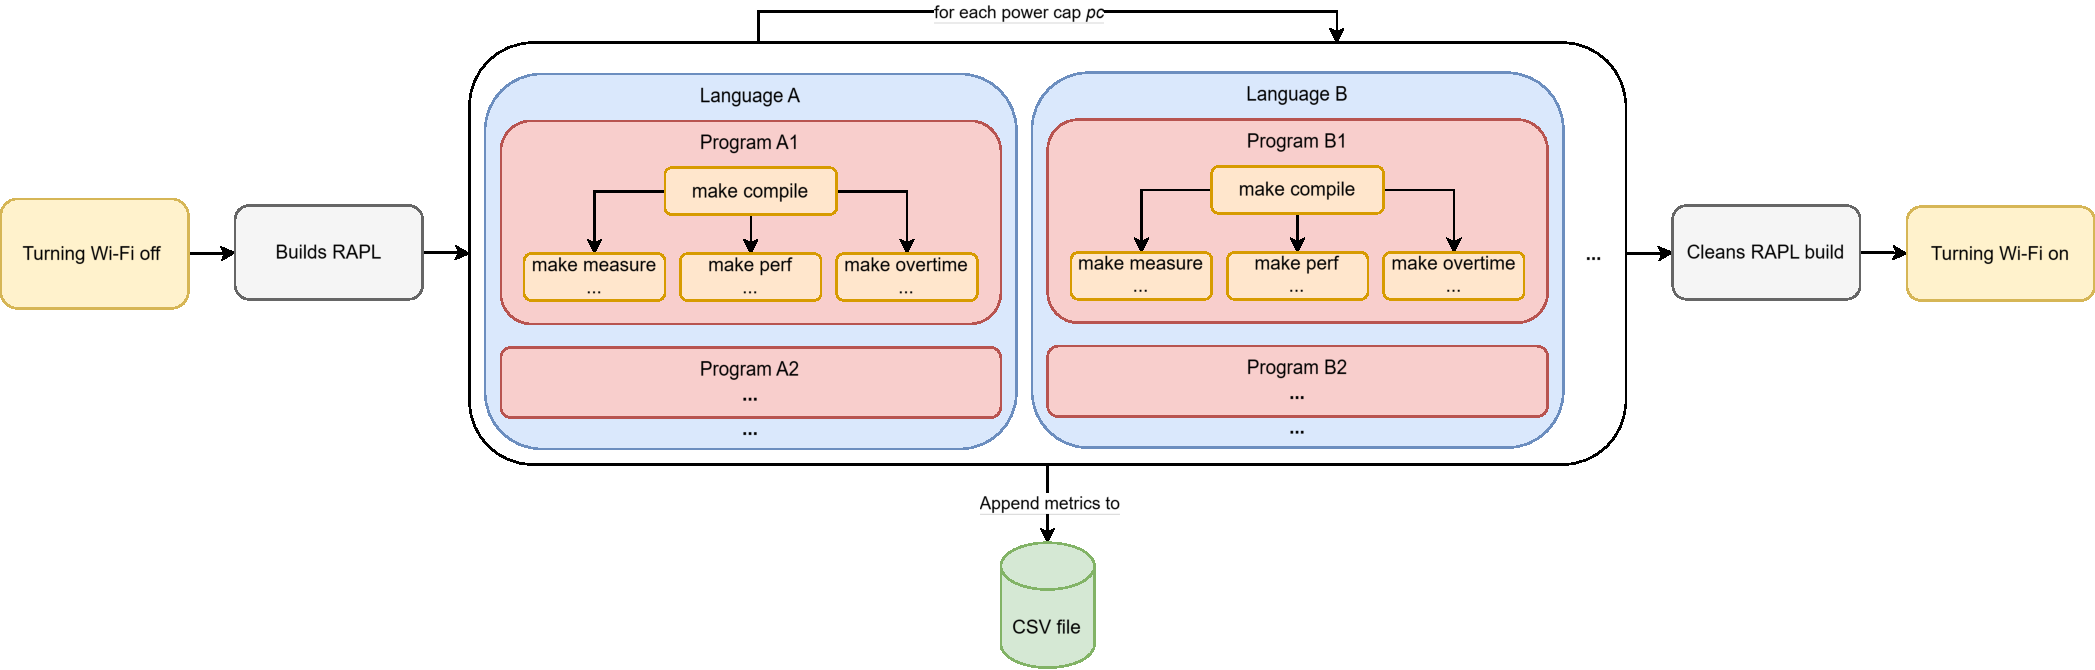
\includegraphics[width=\linewidth]{images/measure_sh.pdf}
    \caption{Running GreenMeasurer through the \texttt{measure.sh} script.}
    \label{measure_sh_diagram}
\end{figure*}

To prevent the need for manual system recovery, \textit{GreenMeasurer} automatically restores Wi-Fi and power settings after each measurement or if the process is interrupted.

\section{Demonstration}
\label{demo_section}

In this section, we demonstrate the use of GreenMeasurer in both calibration modes and for the two types of measurements it can perform while executing the recursive Fibonacci(55) implementation in C. We used this program as a simple example that generates enough computational load to produce stable and comparable energy measurements. Using smaller input values would lead to shorter executions, making the results more sensitive to background system activity and measurement noise.

The machine used for the demonstration was running Linux Ubuntu~22.04, equipped with an Intel(R) Core(TM) i7-8750H processor (6~cores, 12~threads, base clock 2.2~GHz, turbo speed 4.1~GHz), 16~GB of RAM and cache sizes of 384~KB (L1), 1.5~MB (L2) and 9~MB (L3).

All data used in this section can be found in the \texttt{paper\_data} folder of the repository. This includes CSV files containing the results, text files from the power cap and temperature calibrations, and Jupyter Notebook (\texttt{.ipynb}) files used to generate the graphs.

An important aspect of any energy measurement framework is the overhead it introduces during execution. GreenMeasurer performs measurements externally through system calls in C, avoiding modifications to the target program. To estimate the impact of this approach, we refer to the study by Pereira et~al.~\cite{PEREIRA2021102609}, which evaluated an earlier version of this framework. In their experiments, the energy readings obtained through system calls were compared to direct RAPL and jRAPL measurements within program source code. The observed differences were found to be insignificant, indicating that the overhead introduced by this external measurement mechanism is minimal. Although these results were obtained with a previous version, they suggest that the current GreenMeasurer implementation likely introduces negligible measurement overhead as well.


The first step is temperature calibration. To do this, we executed a \textit{sleep 60} command and measured the average temperature afterward. The resulting baseline temperature for subsequent executions was 43.8\textdegree C. Note that the file \texttt{cores\_temperature.txt} contains the complete output of the \textit{sensors} command, but the relevant information is in the last line ("\texttt{Average temperature: 43.8\textdegree C}").

Next, we performed the power cap calibration to determine the optimal power cap value. In this step, we aimed to identify the power cap at which the \textit{Package} power consumption is minimized. We tested power cap settings ranging from 2 W to 25 W using the Python implementation of the Fibonacci algorithm provided in the \texttt{Utils/} folder, with an input value of 40. During this process, we also configured three additional parameters: a time limit of 4~hours for each program execution, a CPU temperature variance threshold of 5\textdegree{}C and the number of repetitions for each program (4 runs).
 The standard output of this calibration, available in the file \texttt{powercap\_report.txt}, summarizes the results. Based on this analysis, we found that a power cap value of \textit{4~W} provides the most efficient balance. Therefore, all subsequent measurements were conducted using this setting. In the following subsections, we present the results for each type of measurement offered by GreenMeasurer. For this purpose, we used the \texttt{measure.sh} Bash script.

\subsection{Standard Measurements}
\label{stdM_results}

To demonstrate how GreenMeasurer can measure the energy consumption and execution time of a software system (referred to here as \textit{standard measurements}), we ran the Fibonacci algorithm in C with an input of 55, both without power capping and with a power cap of 4~W, repeating each configuration 10 times (\textit{n\_times = 10}), with a \textit{time\_out\_limit} of 4~hours and a CPU temperature variance threshold of 5\textdegree C, as defined during the power cap calibration process. Figure~\ref{fig:std} shows the RAPL energy components (\textit{Package}, \textit{Core}, \textit{DRAM} and \textit{GPU}) along with the runtime for all 10 measurements. We observe that applying a power cap reduces the energy consumption of all components but increases the runtime. This behavior was previously reported in~\cite{10.1145/3687997.3695638}, although in that study, energy consumption was measured only at the \textit{Package} level. Our primary goal here is to demonstrate that GreenMeasurer can measure energy components and runtime for software systems, so an in-depth analysis of these results is beyond the scope of this paper.

\begin{figure}[!ht]
    \centering
    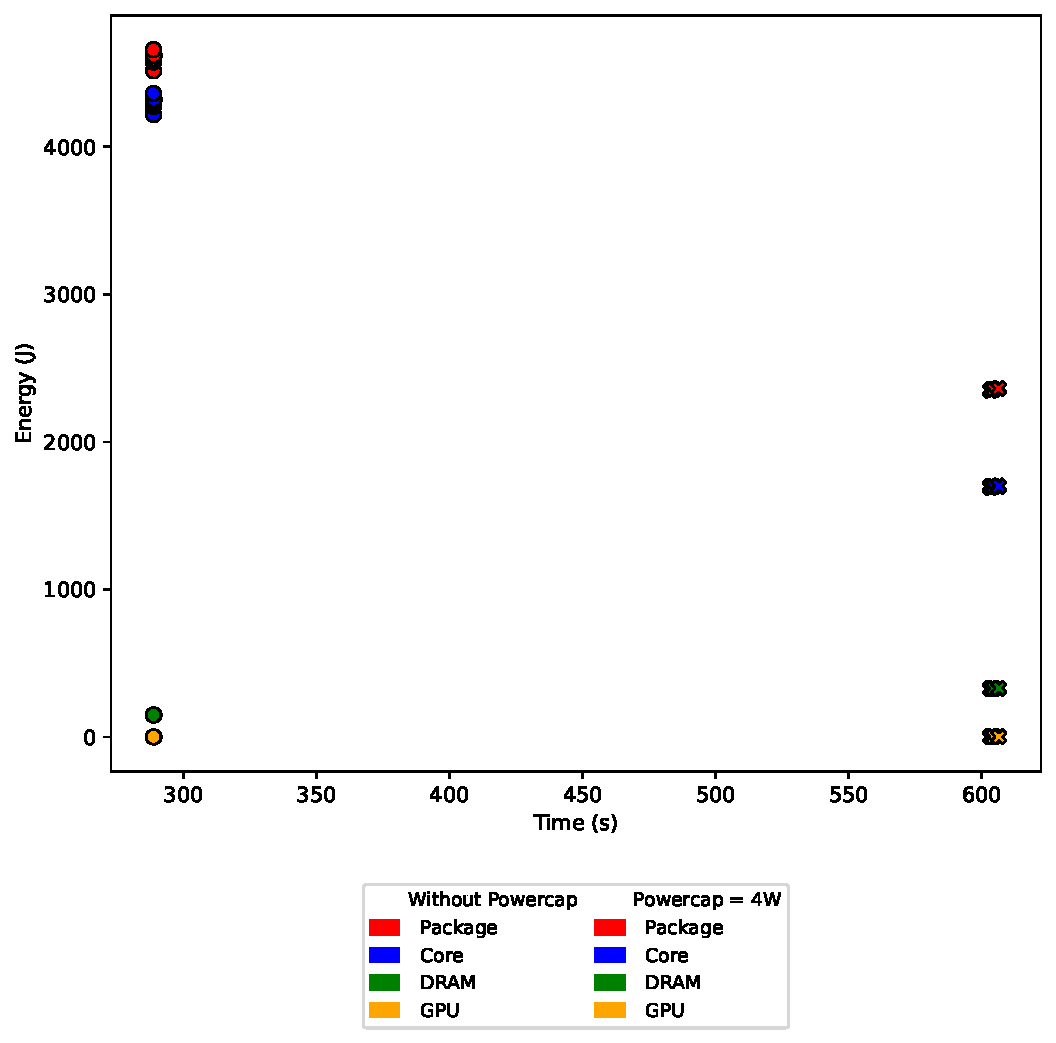
\includegraphics[width=1\linewidth]{images/results/std.pdf}
    \caption{Standard Results for Fibonacci(55) in C}
    \label{fig:std}
\end{figure}

\subsection{Over-Time Measurements}

In this type of measurement, we executed the same Fibonacci program in C using the parameters described in Section~\ref{stdM_results}, except for the number of executions (\textit{n\_times}), which ranged from 10 to 1 for demonstration purposes only. The experiments were conducted both with a 4~W power cap and without any power cap enabled. This setup allows us to compare the four energy counters under consideration throughout the program's execution. As shown in Figure~\ref{fig:Overtime_res}, the CPU temperature increases during execution without a power cap but decreases when the power cap is applied, which is consistent with the expected behavior due to power limitation. Furthermore, the total energy consumption decreases when the power cap is enabled, similarly to what was observed in Section~\ref{stdM_results}. As a suggestion for future researchers, increasing the measurement interval could provide a more detailed view of the results. Overall, these experiments demonstrate that GreenMeasurer can effectively measure both energy consumption and CPU temperature during the execution of a software system.

\begin{figure}[!ht]
    \centering
    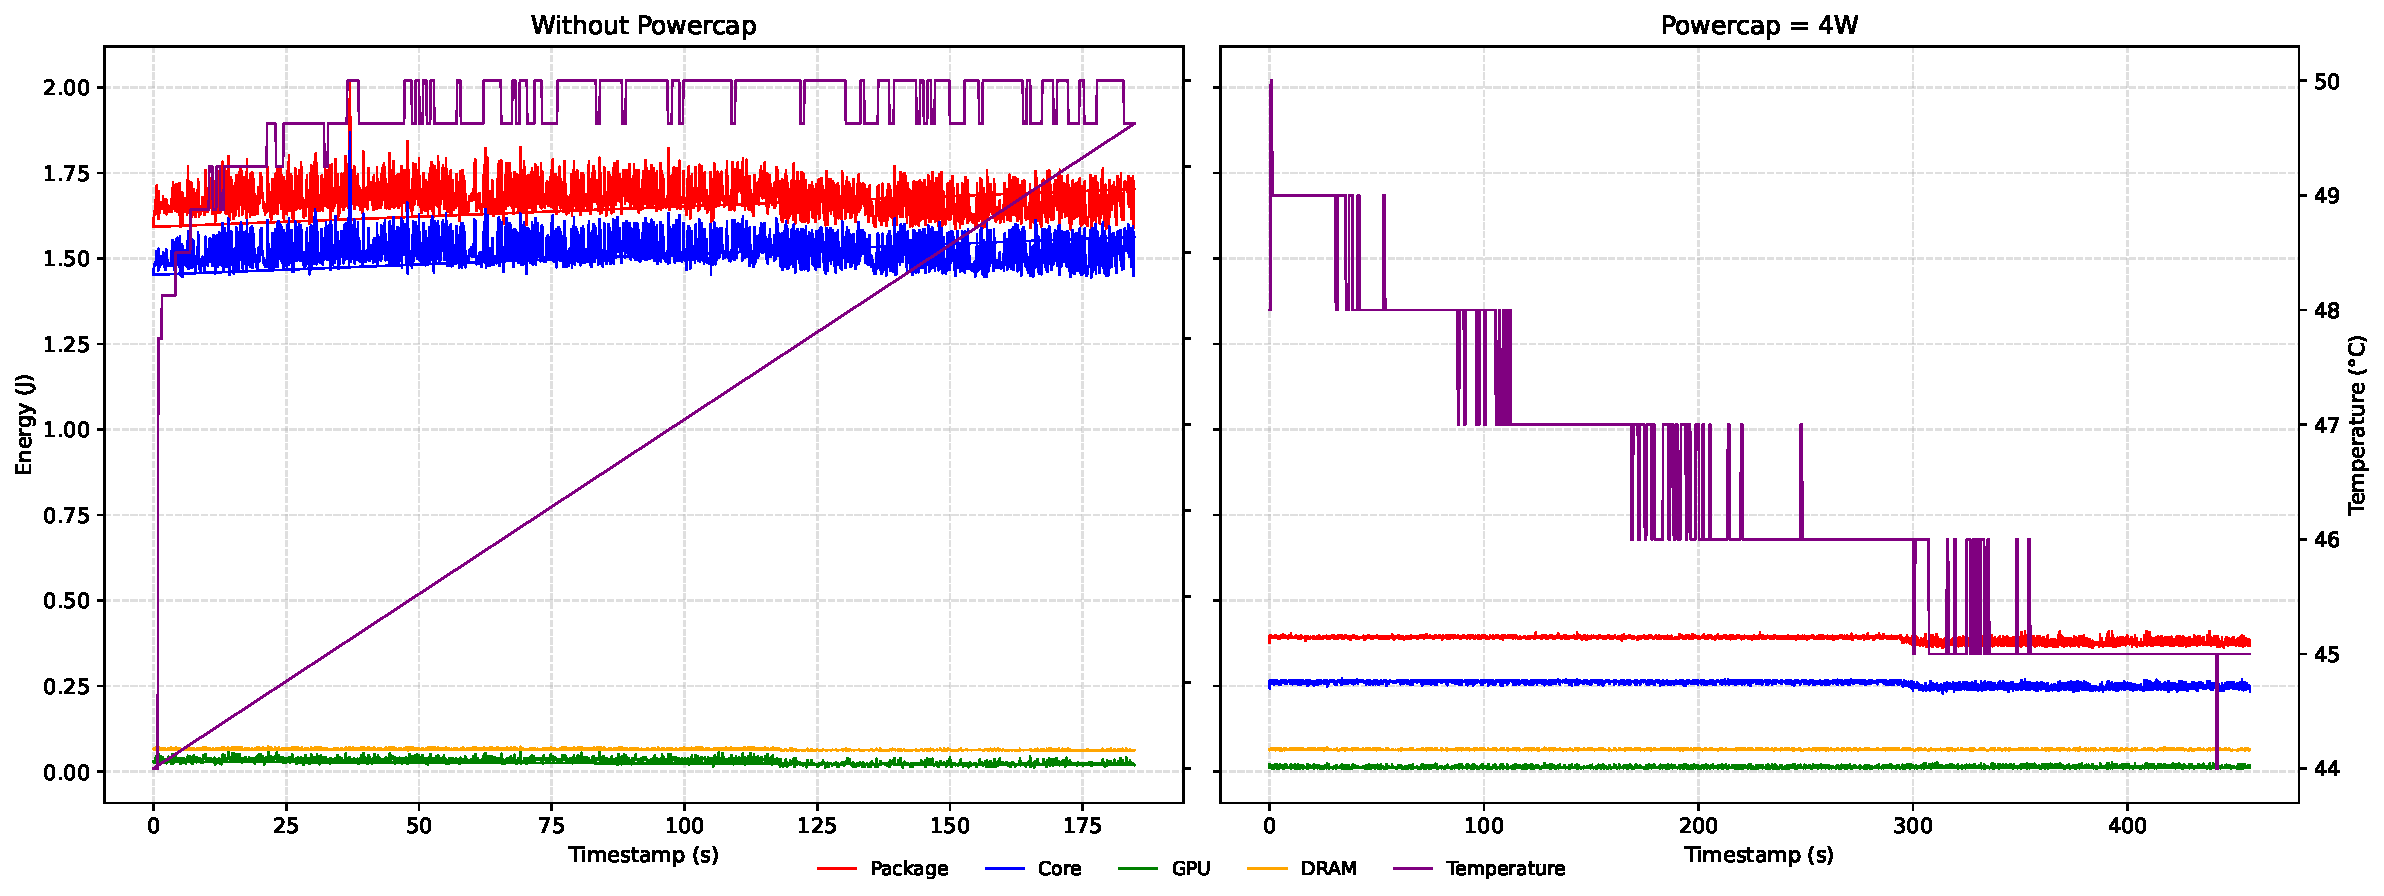
\includegraphics[width=1\linewidth]{images/results/overtime.pdf}
    \caption{Over-time results for Fibonacci(55) in C.}
    \label{fig:Overtime_res}
\end{figure}

\subsection{Evaluation Plan: Comparison with CodeCarbon and EnergiBridge}
\label{sec:eval_plan}

\textbf{[Planned; no results yet.]} The workload is a recursive Fibonacci implementation in Python (\texttt{Languages/Python/Fibonacci}), deterministic and CPU-bound, with an input long enough (several seconds) to make the counters meaningful; the C version can be added to show language independence. GreenMeasurer, EnergiBridge and CodeCarbon are run on the same machine with the same workload, input and number of repetitions (e.g., 30). CodeCarbon wraps the Python call, whereas GreenMeasurer and EnergiBridge run the command externally. The planned experiments are:

\begin{enumerate}
    \item \textit{Standard mode.} Mean, standard deviation and coefficient of variation of energy (J) and time (ms) per tool, with the same system state in all runs and statistical tests of the differences.
    \item \textit{Over-time mode.} Cumulative energy and derived power over time, compared with the time series of the other tools where available, and the final total compared with experiment 1.
    \item \textit{Tool overhead.} Energy and time of the workload with each tool versus without any tool, and of an idle period of the same length.
    \item \textit{Usability and extensibility.} Steps and configuration lines needed to measure the same workload, and the files and lines needed to add a backend (with no change to the core), summarized in a feature table.
    \item \textit{Portability} (depending on the available machines). Experiment 1 on systems with different CPUs, with and without an NVIDIA GPU, reporting which backends were detected and how unsupported ones were reported.
\end{enumerate}

Threats to validity: the counters measure hardware domains and not the process; the tools may read different domains (package, whole system or modelled values), so absolute differences must be explained and not assumed to be errors; and the results are limited to the tested machines. AMD CPUs are not covered.


\section{Conclusions and Future Work}
\label{conc_section}

This paper introduced GreenMeasurer, a lightweight and extensible framework designed to facilitate non-intrusive measurement of energy consumption and runtime performance of software systems on Linux and macOS. The framework reads hardware energy counters through backends (Intel RAPL, NVIDIA NVML and, on macOS, \textit{powermetrics}), selects the CPU and GPU backends independently, reports unsupported metrics explicitly, and incorporates temperature calibration, over-time monitoring and, on Intel CPUs, power capping. Experimental results, including the execution of a Fibonacci algorithm in C, illustrate GreenMeasurer's capability to produce reproducible energy measurements, as well as insights into the impact of power limits on energy consumption and performance metrics. Measurements are hardware-domain measurements, not per-process attributions.

Several limitations remain. The macOS backends are implemented but not yet validated on hardware, the AMD backend is not validated, and the API has no explicit ABI version, so the core and backends must be built from compatible sources. Future work includes validated AMD support, a comparison with CodeCarbon and EnergiBridge (Section~\ref{sec:eval_plan}), a comparison against an external power meter, and support for virtualized environments and further components such as I/O and network.


\section*{Acknowledgment}

This work is funded by national funds 
through FCT - Fundação para a Ciência e a Tecnologia, I.P., under the support 
UID/50014/2025 (\url{https://doi.org/10.54499/UID/50014/2025}).
Simão Cunha is also funded by FCT grant 2025.04596.BDANA (\url{https://doi.org/10.54499/2025.04596.BDANA}).



\bibliographystyle{IEEEtran}
\bibliography{bibliography}


\end{document}
